\section{\ce{[Cu(SCN)_2(4-methoxypyridine)_2]_n}}
\subsection{Synthesis}
0.48 g \ce{Cu(NO_3)_2 * 3 H_2O} (2 mmol), 0.39 g KSCN (4 mmol) and 0.44 g 4-methoxy-pyridine (4 mmol) were mixed with 40 mL distilled \ce{H_{2}O}. Stirring was conducted for 2 hours and 30 minutes at 60$^\circ$C. After filtration the green solution was stirred again for 50 minutes at the same temperature and then cooled down to RT. Over the course of 24 hours green crystals precipitated.
Anal. Calculated for \ce{C_{14}H_{14}CuN_{4}O_{2}S_{2}} (397.96 g/mol) : 42.25\% C; 3.55\% H; 14.08\% N; 16.11\% S;
Found: 41.84 \% C; 3.51\% H; 14.14 \% N; 15.69\% S;
IR (ATR, cm$^{-1}$): 2086 (s), 2072 (s), 1614 (s), 1566 (s), 1512 (s), 1434 (s), 1299 (s), 1205 (s), 1059 (m), 1030 (s), 1012 (m), 844 (m), 817 (s), 732 (w), 659 (w), 573 (w), 535 (s), 464 (s)


\begin{figure}[h!]
\centering
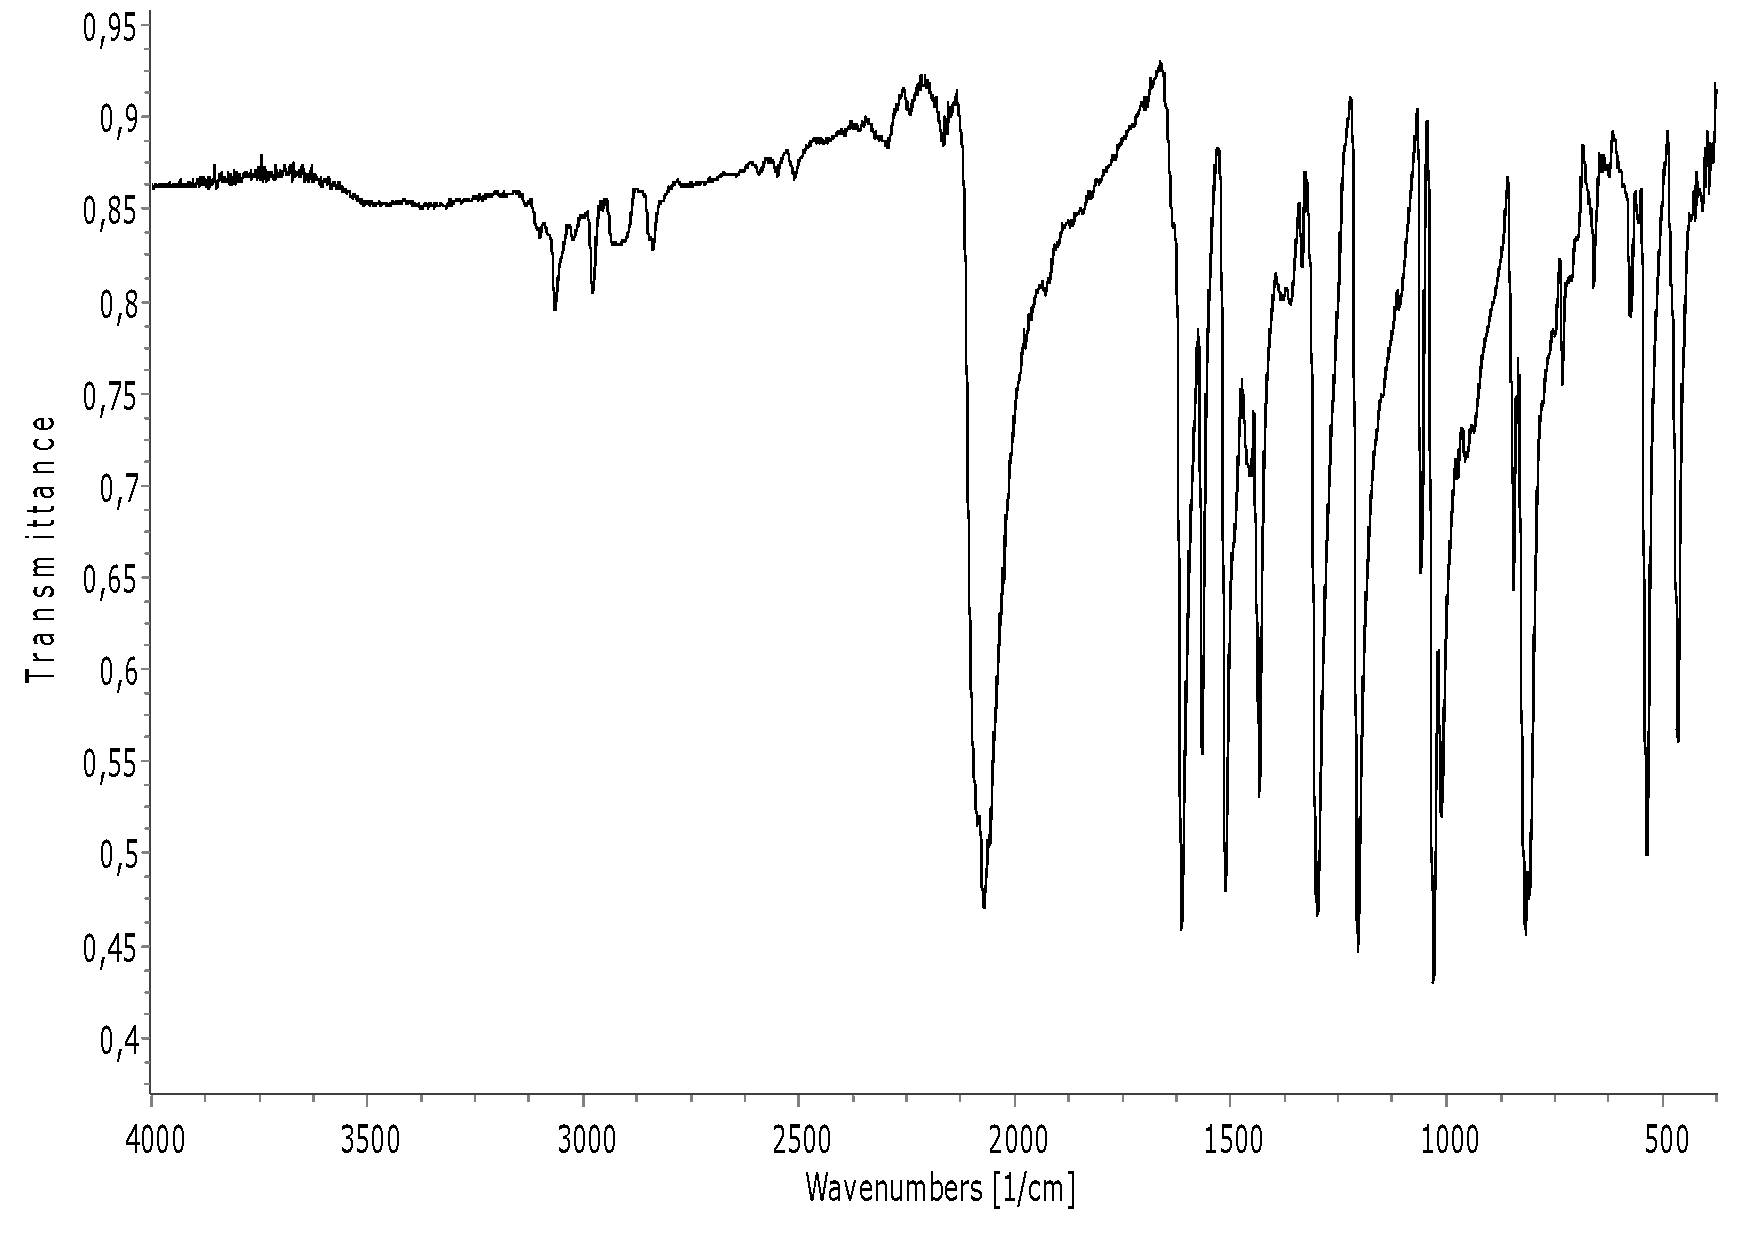
\includegraphics[scale=0.9, width=1\textwidth]{figures/CuR4MOP-IR.pdf}
\caption{IR spectrum of \ce{[Cu(SCN)_2(4-MeOpy)_2]_n}}
\end{figure}

\subsection{Structural characterization}
A perspective view of \ce{[Cu(SCN)_2(4-MeOpy)_2]_n} is given in fig. \ref{fig:CuR4MOP_pv}. The 2D layer system of the Cu-NCS sublattice is displayed in fig. \ref{fig:CuR4MOP_packv}. Table \ref{batlb:CoR4MOP} lists the chosen bond parameters. The three crystallographically independent Cu(II) metal centers in the structure of Cu(SCN)$_2$(4-Me-O-py)$_2$ are located on inversion centers. Taking into account the semi-coordinative Cu-S bond distances, each Cu(II) is bound to four N and two S atoms, whereas two N belong to two 4-MOPs in trans configuration. The remaining 4 atoms each belong to a isothiocyanate anion. The Cu-N(py) bond distances vary from 2.010(3) to 2.037(2) \AA, the Cu-N(NCS) bond distances vary from 1.953(2) to 1.970(3) \AA, whereas the semi-coordinative Cu-S bond lengths are in the range of 2.930(2) to 3.112(2) \AA. The three NCS-groups behave in a different manner. N(2)-C(2)-S(2) acts as N-terminal ligand only, N(1)-C(1)-S(1) acts as  $\mu$(N,S) ligand, to bridge Cu(1) and Cu(3) centers, N(3)-C(3)-S(3) acts as $\mu$(N,S,S’)-bridging ligand to connect all three different metal centers. The 2D system of Cu(SCN)$_2$(4-Me-O-py)$_2$ may be described as polymeric chains of alternating Cu(1) and Cu(3) polyhedra oriented along the c-axis. These chains are formed via di-$\mu$-(N,S) bridging NCS-anions. This is where the Cu(1) polyhedra are further connected by Cu(2) polyhedra along the b-axis of the triclinic unit cell (Fig. \ref{fig:CuR4MOP_packv}). The N(1)-C(1)-S(1) $\mu$(N,S) bridge has a Cu-N\ce{***}S-Cu torsion angle of +64.1$^\circ$, and the N(3)-C(3)-S(3) $\mu$(N,S,S’)-bridge forms Cu-N\ce{***}S-Cu torsion angles of  -27.1 and -165.7$^\circ$. 

\renewcommand{\arraystretch}{1.5}
\begin{table}[htpb!]
\centering
\captionabove{Selected bond lengths (\AA) and angles ($^\circ$) for \ce{[Cu(SCN)_2(4-MeOpy)_2]_n}. Symmetry codes: (') 1-x, -y, 2-z; (*) 1-x, 1-y, -z; ('') 1-x, 2-y, 1-z. }
\begin{tabular}{|l|l|l|l|}
\hline
Cu(1)-N(1') & 1.953(2) & Cu(1)-N(5') & 2.037(2)\\
\hline
Cu(2)-N(2*) & 1.958(3) & Cu(2)-N(6*) & 2.027(2)\\
\hline
Cu(3)-N(3'') & 1.970(3) & Cu(3)-N(7'') & 2.010(3)\\
\hline
N(1)-C(1) & 1.159(4) & C(1)-S(1) & 1.635(3)\\
\hline
N(2)-C(2) & 1.145(4) & C(2)-S(2) & 1.622(4)\\
\hline
N(3)-C(3) & 1.157(4) & C(3)-S(3) & 1.641(3)\\
\hline
\hline
N(1')-Cu(1)-N(5') & 90.87(10) & N(2*)-Cu(2)-N(6*) & 90.16(10)\\
\hline
N(3)-Cu(3)-N(7'') & 90.02(11) & N(21)-Cu(1)-N(11a) & 91.04(9)\\
\hline
Cu(1)-N(1)-C(1) & 162.3(2) & N(1)-C(1)-S(1) & 179.6(3)\\
\hline
Cu(2)-N(2)-C(2) & 155.0(3) &N(2)-C(2)-S(2) & 179.4(3)\\
\hline
Cu(3)-N(3)-C(3) & 168.3(2) & N(3)-C(3)-S(3) & 178.8(3)\\
\hline
\end{tabular}
\label{batlb:CoR4MOP}
\end{table}



\begin{figure}[htpb!]
\centering
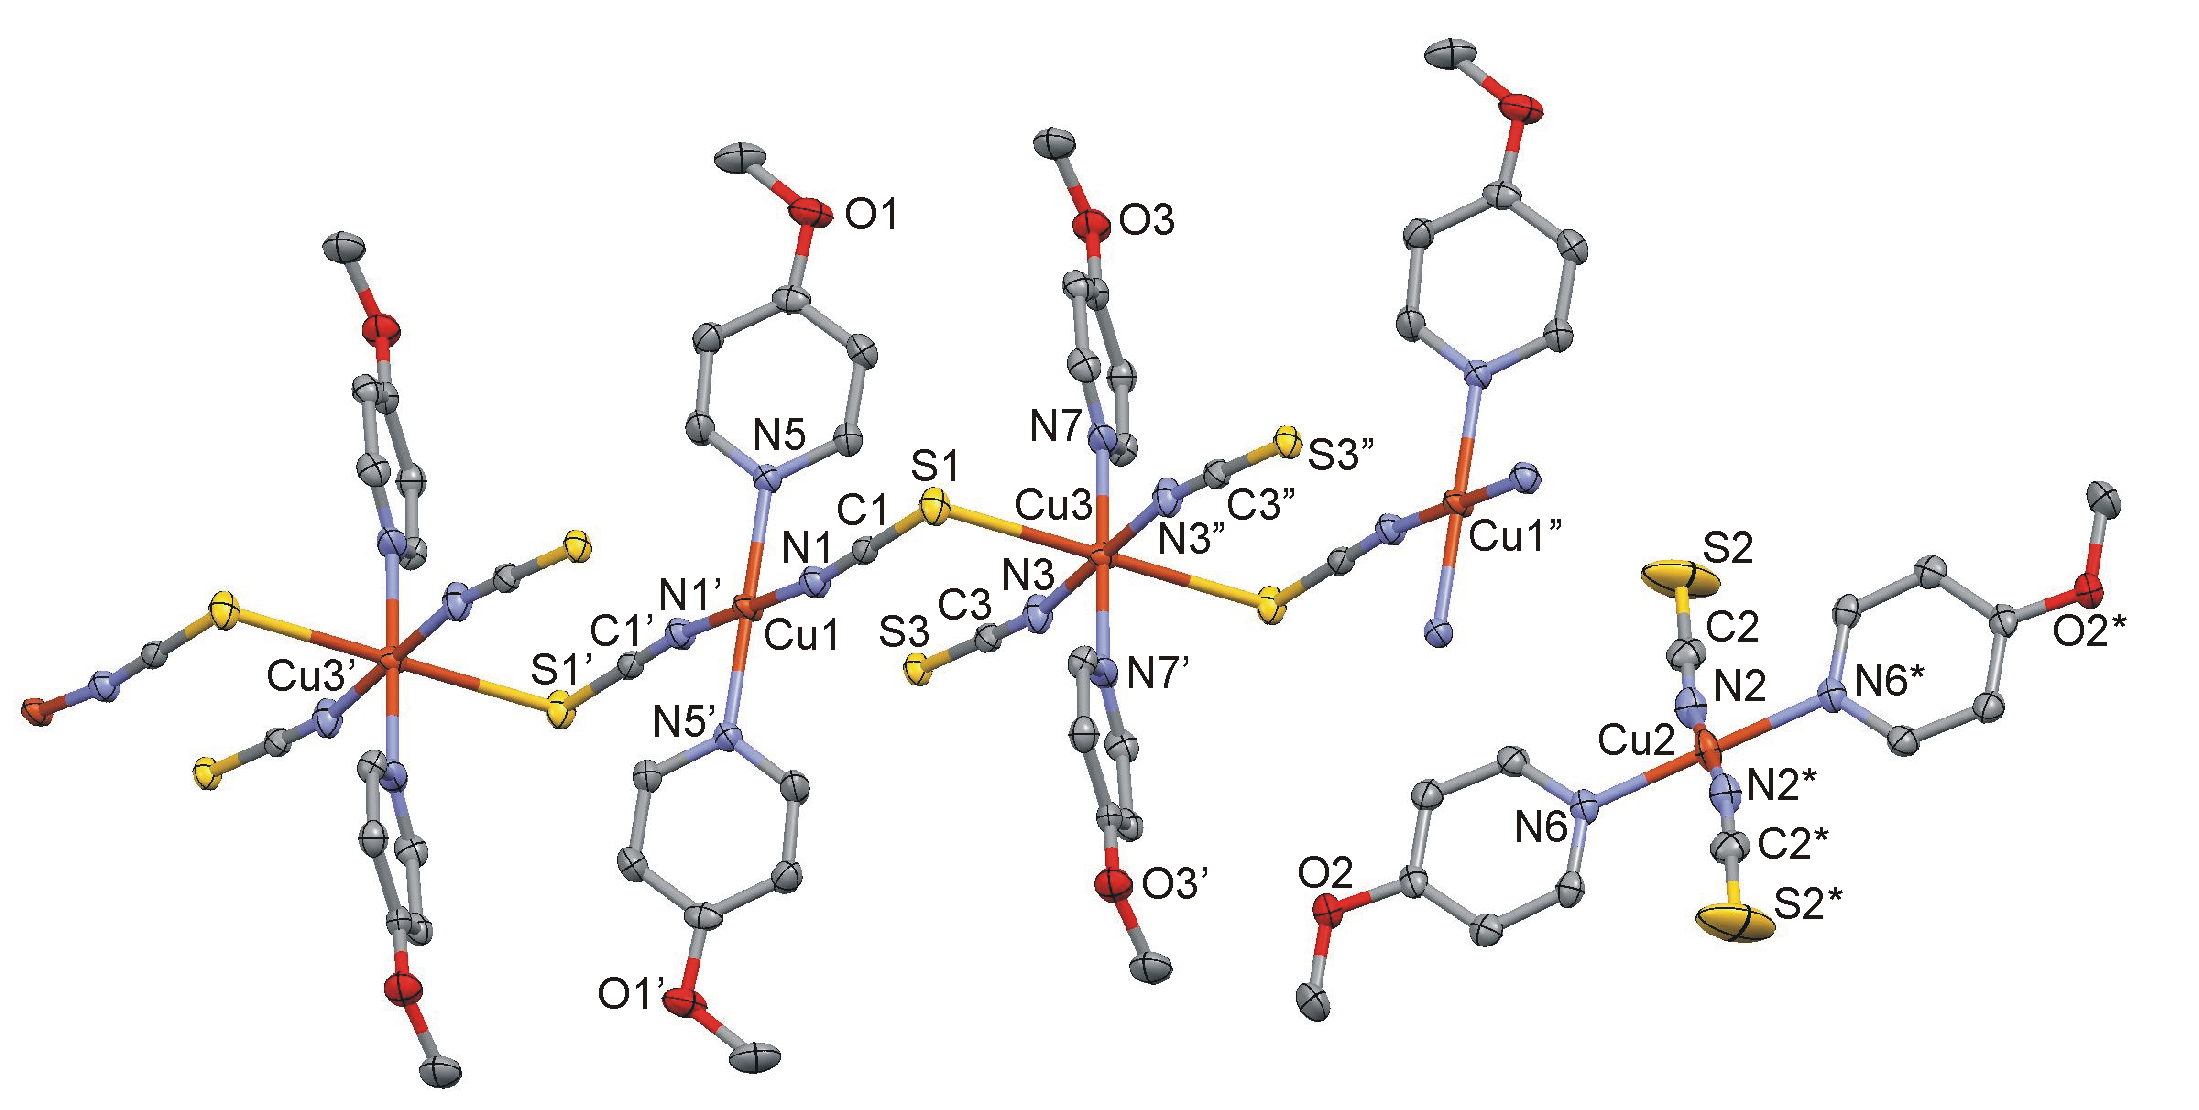
\includegraphics[width=1\textwidth]{figures/curmop_FIGm11.png}
\caption[Perspective view of \ce{[Cu(SCN)_2(4-MeOpy)_2]}]{Perspective view of \ce{[Cu(SCN)_2(4-MeOpy)_2]_n} with the atom numbering scheme. Symmetry codes: (') 1-x, -y, 2-z; (*) 1-x, 1-y, -z; ('') 1-x, 2-y, 1-z.}
\label{fig:CuR4MOP_pv}
\vspace{\floatsep}
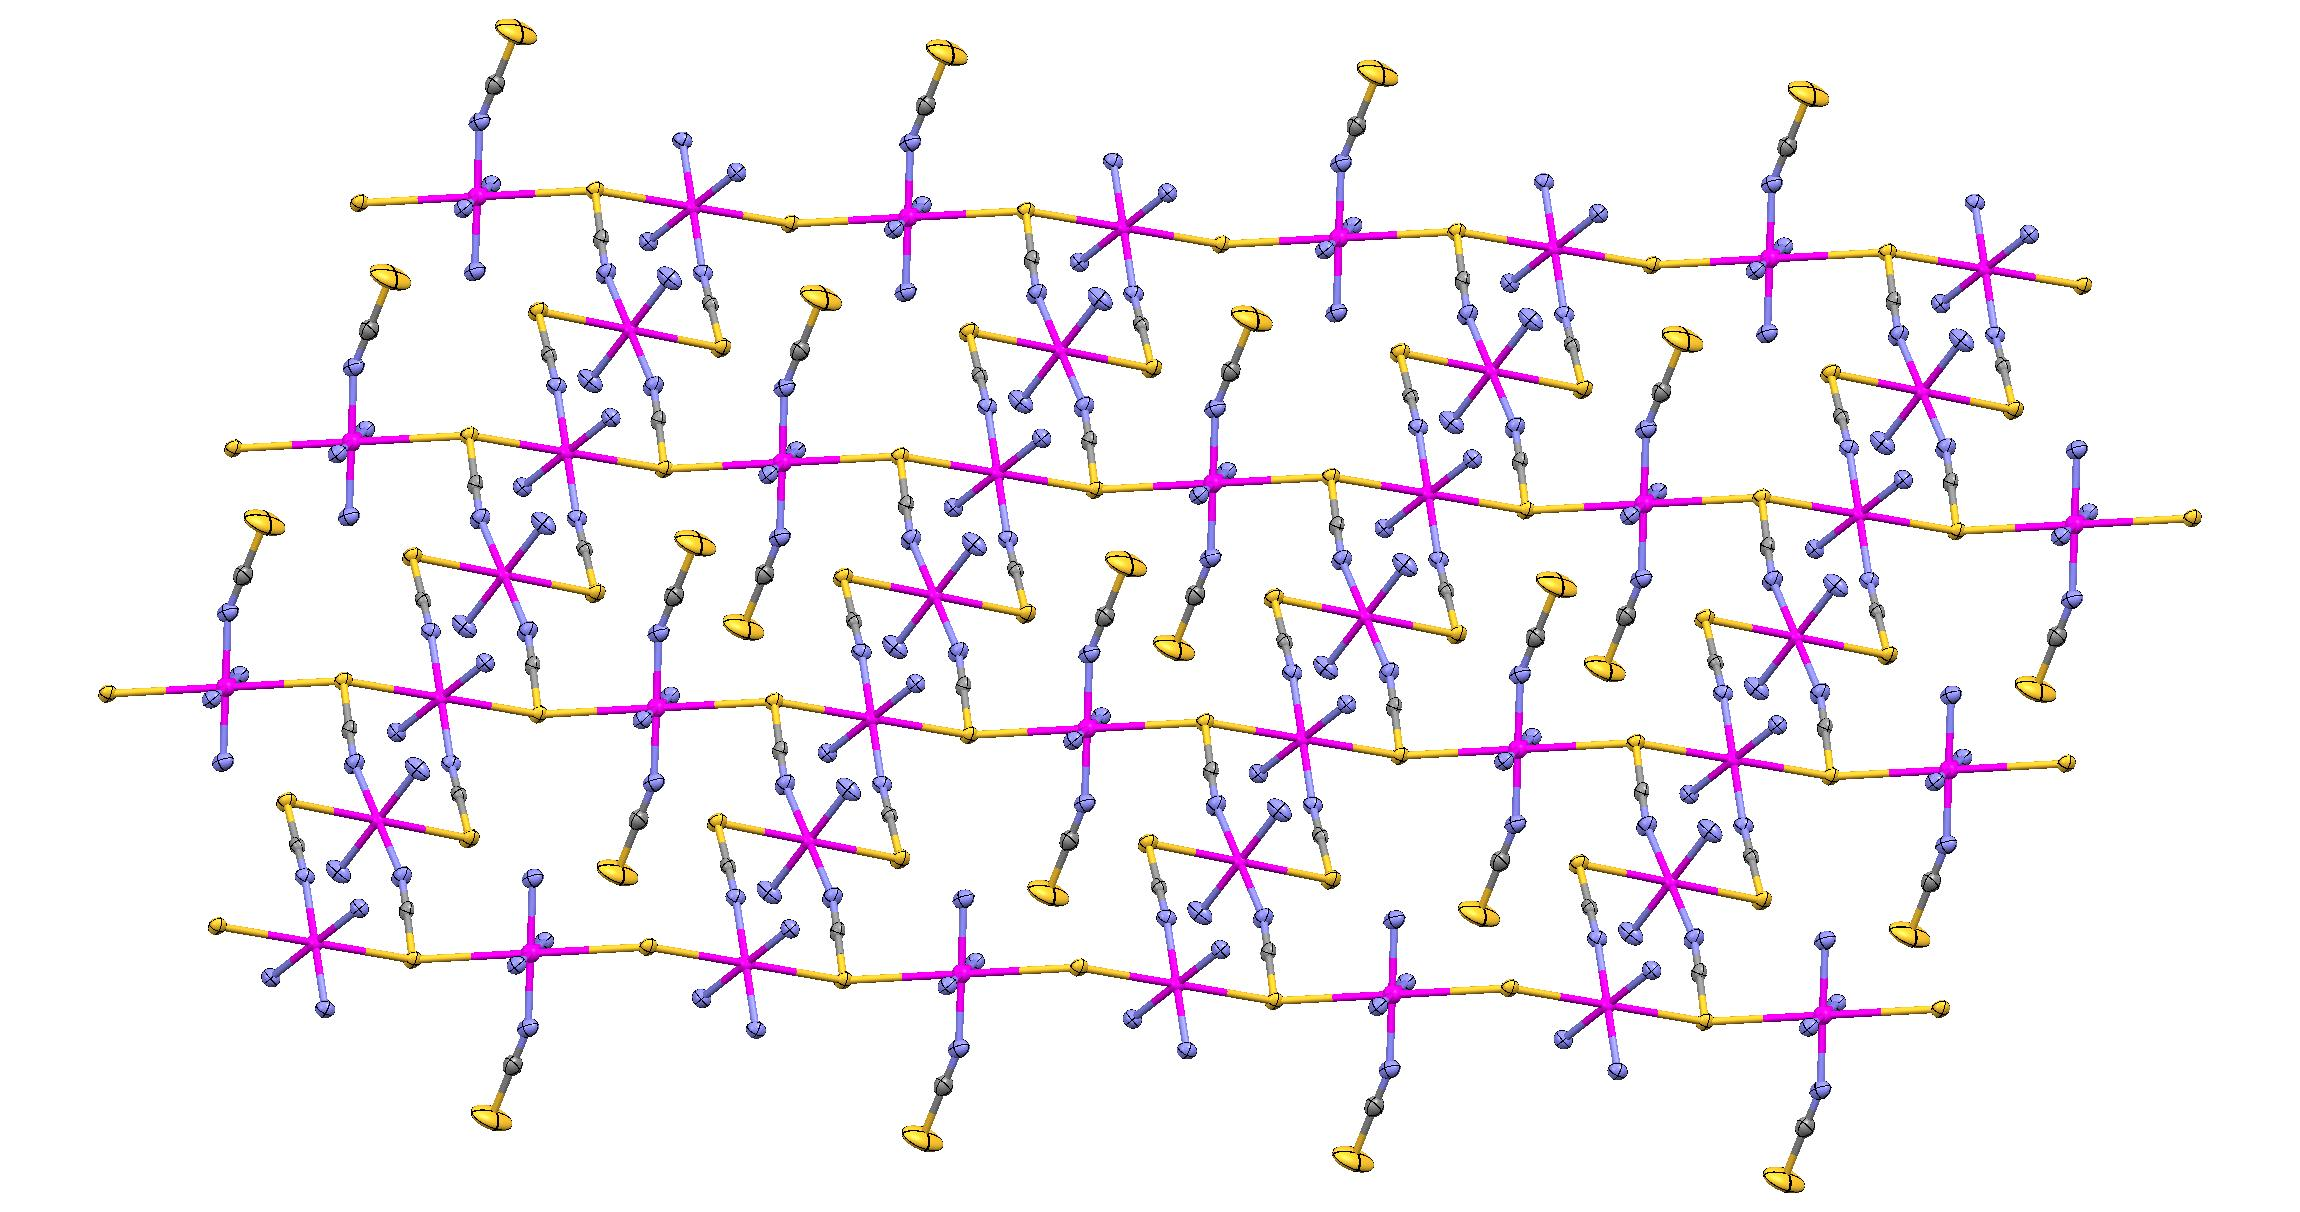
\includegraphics[width=1\textwidth]{figures/curmop_2D.png}
\caption{View onto 2D Cu-NCS sub-lattice of \ce{[Cu(SCN)_2(4-MeOpy)_2]_n}.}
\label{fig:CuR4MOP_packv}
\end{figure}




\begin{table}
\centering
\captionabove{Crystallographic data and processing parameter of \ce{[Cu(SCN)_2(4-MeOpy)_2]_n}}
\begin{tabular}{ | l |  l | }
\hline
Empirical formula & \ce{C_{14}H_{14}CuN_{4}O_{2}S_{2}}\\
\hline
Formula mass & 397.96\\
\hline
System & triclinic\\
\hline
Space group & P-1\\
\hline
a ({\AA}) & 10.981(2)\\
\hline
b ({\AA}) & 11.296(2)\\
\hline
c ({\AA}) & 11.531(2)\\
\hline
$\alpha$ ($^\circ$) & 112.524(3)\\
\hline
$\beta$ ($^\circ$) & 99.366(3)\\
\hline
$\gamma$ ($^\circ$) & 98.311(2)\\
\hline
V (\AA$^{3}) $  & 1269.6(4)\\
\hline
Z & 3\\
\hline
T (K) & 100(2)\\
\hline
$\mu$ (mm$^{-1}$) & 1.549\\
\hline
 D$_{calc}$ (Mg/m$^{3}$) & 1.561\\
\hline
Crystal size (mm) & 0.34 x 0.18 x 0.04\\
\hline
$\theta$ max ($^\circ$) & 26.37\\
\hline
Data collected & 10186\\
\hline
Unique refl./ R$_{int}$ & 5122 / 0.0266\\
\hline
Parameters & 384\\
\hline
Goodness-of-Fit on F$^{2}$ & 1.047\\
\hline
R1 / wR2 (all data) & 0.0410 /0.0998\\
\hline
Residual extrema (e/\AA$^{3}$) & 1.23 /-1.29\\
\hline
\end{tabular}

\label{ptab:CuR4MOP}

\end{table}



